\section{Transformations and push-forward}
\begin{frame}{Transformations of random variables}

\structure{Setup:} 
\begin{itemize}
\item $X$ - random variable with values in $T$ (e.g., $\mR^d$)
\item $P_X$ - distribution of $X$ on $T$
\item $g: T \to U$ - measurable function (transformation)
\item $Y = g(X)$ - transformed random variable with values in $U$
\end{itemize}

\vskip 1em
\structure{Question:} If we know $P_X$, what is the distribution $P_Y$ of $Y = g(X)$?

\vskip 1em
\structure{Examples in ML:}
\begin{itemize}
\item $X \sim \mathcal{N}(0, I)$ (simple), $g$ is neural network, $Y = g(X)$ (complex model distribution)
\item data transformation: $X$ is data, $g$ encodes to latent space
\end{itemize}

\end{frame}

\note[enumerate]
{
\item This is the fundamental question in generative modeling
\item We transform a simple distribution to get a complex one
\item The transformation $g$ is typically a neural network
\item We work directly with distributions on value spaces (as established in Section 2)
\item No need to refer back to abstract probability space $(S, \salg, \mP)$
}


\begin{frame}{Push-forward measure}

\structure{Answer:} distribution of $Y = g(X)$ is the push-forward of $P_X$ by $g$

\vskip 0.5em
\structure{Definition:} $P_Y$ on $U$ defined by
\[
P_Y(C) = P_X(g^{-1}(C)) \quad \text{for } C \subseteq U
\]
where $g^{-1}(C) = \{x \in T: g(x) \in C\}$ is the pre-image

\vskip 1em
\centering
\scalebox{0.55}{
\begin{tikzpicture}[>=Stealth]
% LEFT: domain T with mesh and rectangular g^{-1}(C)
\begin{scope}[shift={(-5,0)}]
    \node at (0,2) {$T$};
    % Mesh (vertical)
    \foreach \x in {-1.5,-1,...,1}
        \draw[gray!70] (\x,-2) -- (\x,2);
    % Mesh (horizontal)
    \foreach \y in {-1.5,-1,...,1.5}
        \draw[gray!70] (-2,\y) -- (1.5,\y);
    % Preimage region g^{-1}(C): ALIGNED WITH GRID
    \fill[blue!25,opacity=0.5] (-1,-1) rectangle (0,1);
    \draw[blue!60,thick] (-1,-1) rectangle (0,1);
    \node[blue!80] at (-0.5,0) {$g^{-1}(C)$};
\end{scope}
% Middle arrow: g
\draw[->,thick] (-2.5,0.5) -- (-0.5,0.5) node[midway,above] {$g: T \to U$};
\draw[<-,thick] (-2.5,-0.5) -- (-0.5,-0.5) node[midway,above] {preimage};
\node at (-1.5,1.8) {\color{carnelian}$P_X(g^{-1}(C)) = P_Y(C)$};
% RIGHT: codomain U with warped mesh + image C
\begin{scope}[shift={(2,0)}]
    \node at (0,2) {$U$};
    % Warped vertical mesh lines
    \foreach \x in {-1.5,-1,...,1}
    \draw[gray!70,domain=-2:2,smooth,variable=\t]
        plot ({0.9*\x + 0.5*sin(\t r)}, {\t + 0.5*sin(\x r)});
    % Warped horizontal mesh lines
    \foreach \y in {-1.5,-1,...,1.5}
    \draw[gray!70,domain=-2:1.5,smooth,variable=\t]
        plot ({0.9*\t + 0.5*sin(\y r)}, {\y + 0.5*sin(\t r)});
    % Image region C
    \begin{scope}
        \fill[blue!25,opacity=0.5]
            plot[domain=-1:0,smooth,variable=\x]
                ({0.9*\x + 0.5*sin(-1 r)}, {-1 + 0.5*sin(\x r)})
            -- plot[domain=-1:1,smooth,variable=\y]
                ({0.9*0 + 0.5*sin(\y r)}, {\y + 0.5*sin(0 r)})
            -- plot[domain=0:-1,smooth,variable=\x]
                ({0.9*\x + 0.5*sin(1 r)}, {1 + 0.5*sin(\x r)})
            -- plot[domain=1:-1,smooth,variable=\y]
                ({0.9*(-1) + 0.5*sin(\y r)}, {\y + 0.5*sin(-1 r)})
            -- cycle;
        \draw[blue!60,thick]
            plot[domain=-1:0,smooth,variable=\x]
                ({0.9*\x + 0.5*sin(-1 r)}, {-1 + 0.5*sin(\x r)})
            -- plot[domain=-1:1,smooth,variable=\y]
                ({0.9*0 + 0.5*sin(\y r)}, {\y + 0.5*sin(0 r)})
            -- plot[domain=0:-1,smooth,variable=\x]
                ({0.9*\x + 0.5*sin(1 r)}, {1 + 0.5*sin(\x r)})
            -- plot[domain=1:-1,smooth,variable=\y]
                ({0.9*(-1) + 0.5*sin(\y r)}, {\y + 0.5*sin(-1 r)})
            -- cycle;
        \node[blue!80] at (-0.4,-0.1) {$C$};
    \end{scope}
\end{scope}
\end{tikzpicture}
}

\vskip 0.5em
\structure{Intuition:} probability of $Y$ landing in $C$ equals probability of $X$ being in pre-image

\end{frame}

\note[enumerate]
{
\item Push-forward is how distributions transform under functions
\item The pre-image $g^{-1}(C)$ is the set of points in $T$ that map to $C$
\item Diagram shows: regular grid in $T$ becomes warped in $U$, but probability is preserved
\item This is well-defined because $g$ is measurable
\item In ML: $g$ is neural network, $P_X$ is simple distribution (e.g., Gaussian), $P_Y$ is complex model distribution
\item We're working directly with distributions $P_X$ and $P_Y$, not going back to abstract probability space
}

\begin{frame}{Example: uniform distribution and affine transformation}

\structure{Setup:} $X \sim \text{Uniform}[0, 1]$, transformation $g(x) = 2x + 3$, find distribution of $Y = g(X)$

\vskip 1em
\centering
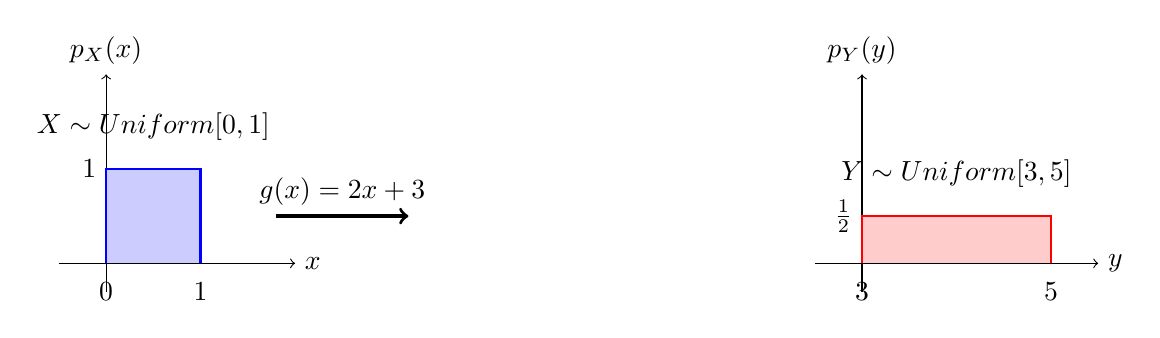
\begin{tikzpicture}[scale=1.2]
% Left: X ~ Uniform[0,1]
\begin{scope}[shift={(-4,0)}]
    % Axis
    \draw[->] (-0.5,0) -- (2,0) node[right] {$x$};
    \draw[->] (0,-0.3) -- (0,2) node[above] {$p_X(x)$};
    
    % Uniform distribution on [0,1]
    \fill[blue!20] (0,0) rectangle (1,1);
    \draw[blue,thick] (0,0) -- (0,1) -- (1,1) -- (1,0);
    
    % Labels
    \node[below] at (0,-0.1) {$0$};
    \node[below] at (1,-0.1) {$1$};
    \node[left] at (0,1) {$1$};
    \node[above] at (0.5,1.2) {$X \sim \text{Uniform}[0,1]$};
\end{scope}

% Arrow with transformation
\draw[->,very thick] (-2.2,0.5) -- (-0.8,0.5) node[midway,above] {$g(x) = 2x+3$};

% Right: Y ~ Uniform[3,5]
\begin{scope}[shift={(1,0)}]
    % Axis
    \draw[->] (2.5,0) -- (5.5,0) node[right] {$y$};
    \draw[->] (3,-0.3) -- (3,2) node[above] {$p_Y(y)$};
    
    % Uniform distribution on [3,5]
    \fill[red!20] (3,0) rectangle (5,0.5);
    \draw[red,thick] (3,0) -- (3,0.5) -- (5,0.5) -- (5,0);
    
    % Labels
    \node[below] at (3,-0.1) {$3$};
    \node[below] at (5,-0.1) {$5$};
    \node[left] at (3,0.5) {$\frac{1}{2}$};
    \node[above] at (4,0.7) {$Y \sim \text{Uniform}[3,5]$};
\end{scope}
\end{tikzpicture}

\vskip 1em
\structure{What happened:}
\begin{itemize}
\item interval $[0,1] \to [3,5]$: shifted by 3, scaled by 2
\item height: $1 \to \frac{1}{2}$: density compressed (probability conserved!)
\end{itemize}

\end{frame}

\note[enumerate]
{
\item This is a simple concrete example showing push-forward
\item The preimage calculation: solve $a \leq 2x+3 \leq b$ for $x$
\item Uniform on $[0,1]$: $P_X([a,b]) = b - a$ when $[a,b] \subseteq [0,1]$
\item After transformation: still uniform, but on $[3,5]$ instead of $[0,1]$
\item The scaling factor 2 will become important when we look at densities (Jacobian)
\item This example shows: push-forward preserves the "shape" but changes location and scale
}
